\documentclass[11pt,a4paper]{article}
\usepackage[T1]{fontenc}
\usepackage[utf8]{inputenc}
\usepackage{lmodern,microtype,graphicx,booktabs,tabularx,array,amsmath,amssymb}
\usepackage[margin=22mm]{geometry}
\usepackage[colorlinks=true,linkcolor=black,citecolor=black,urlcolor=blue]{hyperref}
\usepackage[numbers,sort&compress]{natbib}
\usepackage{caption,float}
\usepackage[section]{placeins}
\captionsetup{font=small,labelfont=bf}
\renewcommand{\topfraction}{0.95}
\renewcommand{\bottomfraction}{0.9}
\renewcommand{\textfraction}{0.05}
\renewcommand{\floatpagefraction}{0.8}
\widowpenalty=10000
\clubpenalty=10000
\setlength{\parskip}{4pt}
\setlength{\parindent}{12pt}
\setlength{\emergencystretch}{1.5em}
\newcommand{\co}{CO\textsubscript{2}}
\newcommand{\rr}{CO\textsubscript{2}RR}
\newcommand{\ca}{Cu--Au}
\title{An agentic framework for X-ray absorption spectroscopy of catalytic interfaces}
\author{Haili Jia and Maria K. Y. Chan\thanks{Corresponding author. E-mail: \href{mailto:mchan@anl.gov}{mchan@anl.gov}.}\\[0.6em]
\small Center for Nanoscale Materials, Argonne National Laboratory,\\
\small 9700 South Cass Avenue, Lemont, Illinois 60439, United States}
\hypersetup{pdftitle={An agentic framework for X-ray absorption spectroscopy of catalytic interfaces},pdfauthor={Haili Jia and Maria K. Y. Chan}}
\date{}
\begin{document}
\maketitle
\begin{abstract}
Designing selective catalysts requires understanding how local atomic environments stabilize intermediates and redirect competing reaction pathways. X-ray absorption spectroscopy (XAS), including in situ and operando measurements, can follow changes in a working catalyst, but assigning its ensemble-averaged response to specific interfacial states requires reliable structural references. Experimentally labeled spectra are scarce for complex interfaces and transient adsorbates, leaving many proposed intermediates difficult to evaluate. Here we present an agentic framework that bridges this gap by connecting controlled atomistic hypotheses to simulated spectra and automated inference. The workflow translates a catalytic question into interface construction, first-principles relaxation, supercomputer-based XAS calculations, AI-ready records, and machine-learning analysis. We demonstrate the framework for electrochemical CO\textsubscript{2} reduction (CO\textsubscript{2}RR), where coadsorption, hydrogenation, and C--C coupling generate competing interfacial states. Cu--Au models vary adsorbate identity, binding geometry, coverage, and distance from the interface. Models trained entirely through the agent identify adsorbates from simulated Cu K-edge spectra with a micro F1 score of 0.78; layer-resolved analysis reveals how deeper metal contributions dilute surface information. A matched adjacent-CO/OCCO design specifies a test of spectral sensitivity to C--C bonding and interface location. By preserving the connection between chemical alternatives and their predicted signals, the framework supports spectroscopic evaluation of catalytic hypotheses and selection of informative subsequent calculations.
\end{abstract}

\section{Introduction}
Improving catalytic selectivity requires identifying the atomic environments and intermediates that direct a reaction toward a desired product. Electrochemical CO\textsubscript{2} reduction (CO\textsubscript{2}RR) makes this challenge particularly acute: formation of ethylene or ethanol requires an overall transfer of 12 electrons per product molecule, while formation of n-propanol requires 18.\cite{ni2024,francis2018} These transfers occur through a network of adsorption, protonation, and bond-forming events whose branching depends on the catalyst and reaction environment. Distinguishing adsorbed CO from its hydrogenated or C--C-coupled derivatives is therefore central to evaluating proposed pathways.\cite{zhan2024,montoya2015}

The relevant catalyst structure must be established during operation. Applied potential, adsorbate coverage, and contact with the electrolyte can change the metal surface and its chemical state. Characterization performed only before or after reaction can miss these transformations. In situ measurements probe a catalyst within a controlled reaction environment; operando measurements additionally relate its state to simultaneously measured catalytic performance.\cite{operando2021} Time-resolved XAS during CO\textsubscript{2}RR, for example, has connected evolving Cu chemical states with product formation.\cite{lin2020}

XAS is especially useful because its element specificity and sensitivity to local coordination and electronic structure do not require long-range crystallinity. Hard X-rays can access catalysts inside electrochemical cells, allowing changes in oxidation state and metal environments to be followed during reaction.\cite{operando2021,lin2020} The interpretation remains challenging because the measured signal combines inequivalent absorbers: a small population near an adsorbate or interface may be obscured by the much larger metal background. A pathway hypothesis therefore requires more than assigning an oxidation state; it requires establishing whether the proposed intermediate and its local environment have a distinguishable spectral response.

Bimetallic interfaces offer useful catalytic functions while increasing the number of plausible local environments. Au--Cu tandem catalysts combine CO formation on Au with further reduction on Cu.\cite{morales2018} The resulting CO population and its proximity to Cu sites motivate a specific question: can XAS distinguish two neighboring CO molecules from a bonded OCCO intermediate, and does that contrast change near Au? The answer depends on local metal coordination, distance from the interface, molecular orientation, and spectator species. These variables must be controlled before a spectral difference can be attributed to a particular chemical step.

Reliable experimental spectrum--structure pairs can support this analysis, but independently labeling every transient adsorbate and interfacial geometry is difficult. Simulations provide an alternative source of labeled data and enable comparisons in which composition, coverage, or location is deliberately held fixed. Available approaches include real-space multiple scattering in FEFF, Green-function or finite-difference calculations in FDMNES, supercell core-excitation methods in VASP, and electron--hole treatments in OCEAN.\cite{rehr2010,joly2001,vasp1996,vaspxas,ocean2011} Choices of absorber ensemble, core-hole treatment, spatial extent, convergence, and processing affect the predicted spectral response. Incorrect adsorption geometry, propagation of an unrelaxed structure, or loss of chemical identity during calculation can consequently change the inferred chemistry, even when a calculation terminates successfully. The problem is both computational scale and scientific consistency.

These labeled spectra also make the inverse problem accessible to machine learning. Neural networks have reconstructed structural distributions from EXAFS and inferred local descriptors of bimetallic catalysts from XANES.\cite{timoshenko2018,marcella2020} Random forests have related near-edge spectra to coordination, mean nearest-neighbor distance, and Bader charge,\cite{torrisi2020} while convolutional neural networks have extracted bond-length information from molecular XAS.\cite{david2023} The appropriate model and target therefore depend on the physical question and the structural diversity represented in training. Featurization controls which spectral variations are retained and can improve robustness to differences between calculated and measured spectra.\cite{chen2024} Multimodal learning further combines complementary edges to infer local composition and defects that may be ambiguous in a single channel.\cite{jia2026}

For catalytic interfaces, realizing these capabilities requires a consistent link between the structural alternatives, their spectra, and the targets learned by the model. A classifier cannot distinguish competing intermediates if relaxation has changed their connectivity without updating the labels; nor can validation establish transfer if related spectra from one geometry appear in both training and testing. The computational workflow must therefore preserve chemical identity and sample independence as carefully as it manages numerical calculations. This requirement links structure generation, simulation, and inference into one scientific task.

Advances in language-model reasoning and tool use make it possible to coordinate this task through a scientific request, reducing repeated manual setup and the need to navigate each software interface separately. Chemistry agents can translate scientific requests into specialized computational actions,\cite{bran2024} while work on automated research platforms emphasizes the need to connect planning, execution, and interpretation through explicit interfaces.\cite{canty2023} Related agentic systems have automated structure preparation, high-performance-computing execution, and analysis for atomistic simulations.\cite{vriza2026} XAS adds the need to connect each chemical state to a specified absorbing-site ensemble and spectral representation. Here the objective is an end-to-end spectroscopy workflow in which the catalytic question remains connected to the structures, supercomputer calculations, and subsequent analysis. Chemical validation and numerical checks are essential because efficient execution alone cannot establish a chemically meaningful result.

We present such a framework for XAS of catalytic interfaces and demonstrate it with Cu--Au models relevant to CO\textsubscript{2}RR. The calculation agent connects natural-language requests to interface construction, relaxation, and XAS on NERSC; linked records feed an automated inference stage. The completed study tests two requirements for hypothesis-driven analysis: whether Cu K-edge spectra contain information about adsorbate identity and whether that information survives the inclusion of deeper Cu layers. A matched adjacent-CO/OCCO design then specifies how the workflow can test a C--C-coupling hypothesis at interface and terrace sites. The identity benchmark establishes spectral sensitivity within the simulated cohort; the matched design defines the next chemically controlled test.

\section{An agentic workflow for interface spectroscopy}
\subsection{Turning a catalytic hypothesis into a computational comparison}
The workflow begins with alternatives that a spectrum should distinguish, rather than with a fixed catalogue of calculations (Fig.~\ref{fig:framework}). For CO coupling at Cu--Au, the alternatives are neighboring CO molecules and a C--C-bonded intermediate. A useful comparison must hold elemental loading and the parent surface fixed while changing connectivity or interface location. The agent translates this intent into structured construction and calculation tasks. Dedicated scientific tools enforce the requested composition, adsorption region, and numerical settings, allowing the scientific question to remain explicit as it moves between different simulation codes.

\begin{figure}[!htbp]
\centering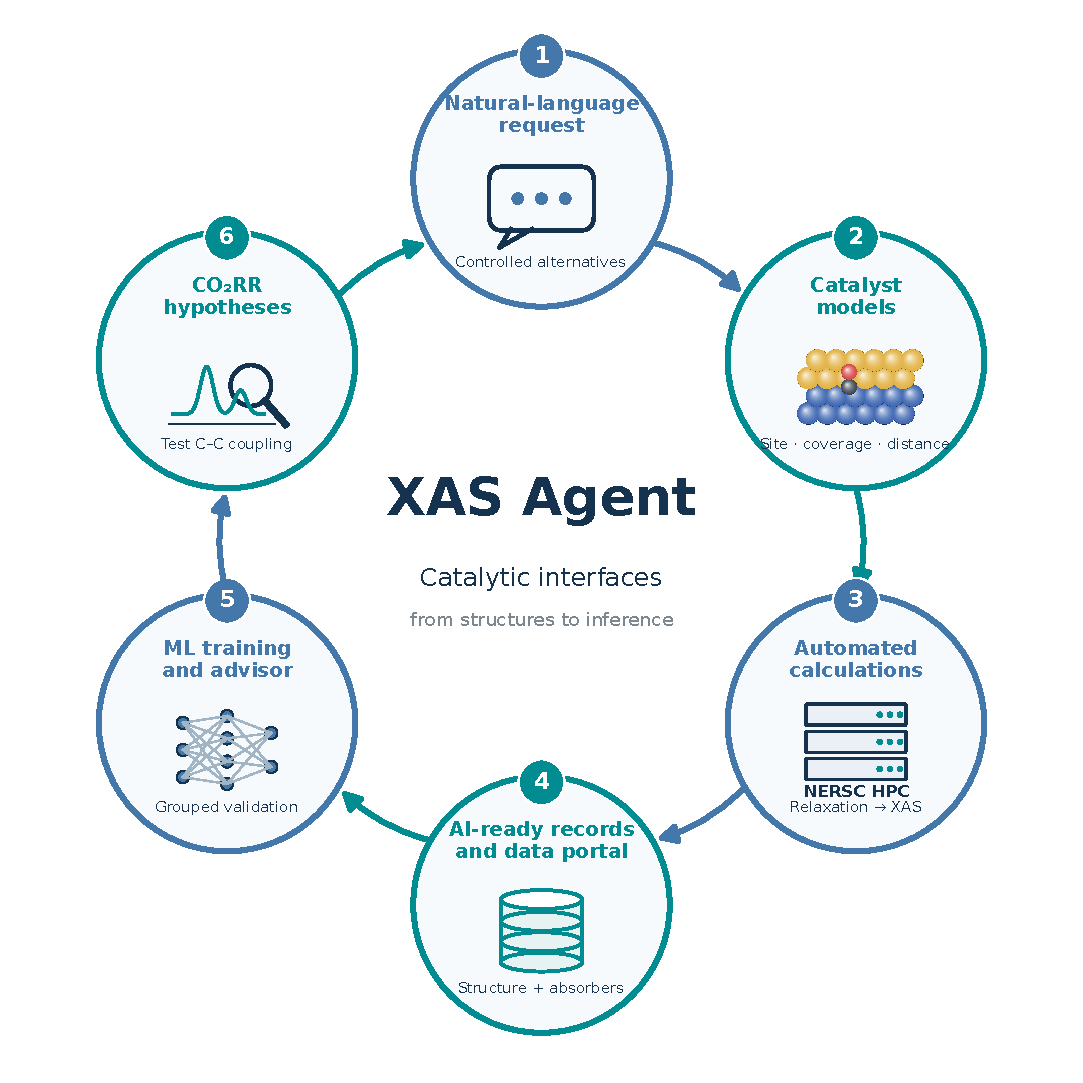
\includegraphics[width=.92\linewidth]{figures/Figure_1_framework.pdf}
\caption{Hypothesis-driven workflow for catalytic XAS. A scientific request specifies structural alternatives that are generated, relaxed, and evaluated by spectroscopy calculations. The calculation agent manages NERSC execution, and AI-ready records connect the outputs to model training and spectral interpretation. The return arrow represents refinement of the next calculation or hypothesis; it does not imply that a closed-loop catalytic discovery experiment has been completed.}
\label{fig:framework}
\end{figure}

The calculation agent directly manages remote work on the National Energy Research Scientific Computing Center (NERSC) Perlmutter supercomputer. After the user supplies access, allocation, and calculation settings, it can prepare job inputs, transfer files, submit and monitor scheduler jobs, and advance from successful relaxation to XAS. Persistent workflow state supports monitoring and recovery without maintaining an active chat session.\cite{nersc} This design reduces repeated manual file handling and scheduler interaction. Routine transfers, submissions, and monitoring therefore proceed with minimal manual intervention once the workflow is configured, while scientific choices and exceptional failures can be reviewed.

Relaxation is a scientific checkpoint because it determines which chemical state is actually probed. The spectrum is generated from the relaxed geometry, and the resulting record preserves the absorber ensemble and observed adsorbate identity. This prevents a requested OCCO starting model that separates into CO from being interpreted as evidence for a coupled state. The calculation stage and the dedicated analysis interface together cover model generation through predictive evaluation; automatic selection of the next catalytic experiment is a subsequent use of their outputs.

\subsection{Representing interfacial chemical space}
At a bimetallic interface, nominal composition alone cannot identify the environment responsible for a spectral change. CO bound to three Cu atoms and CO bound to one Cu and two Au atoms experience different local coordination even on the same parent surface. Conversely, an all-Cu binding motif can lie either near the boundary or on a Cu terrace. To distinguish these effects, each construction specifies the parent surface, the metal atoms defining the adsorption site, and the adsorbate's distance from the nearest interface (Fig.~\ref{fig:dataset}). The extended-surface illustration includes Cu and Au atop sites, Cu--Cu and boundary-spanning Cu--Au bridges, and CuCuCu, CuCuAu, and CuAuAu hollows. These configurations allow changes in local composition to be examined separately from changes in binding multiplicity or interface proximity.

\begin{figure}[!htbp]
\centering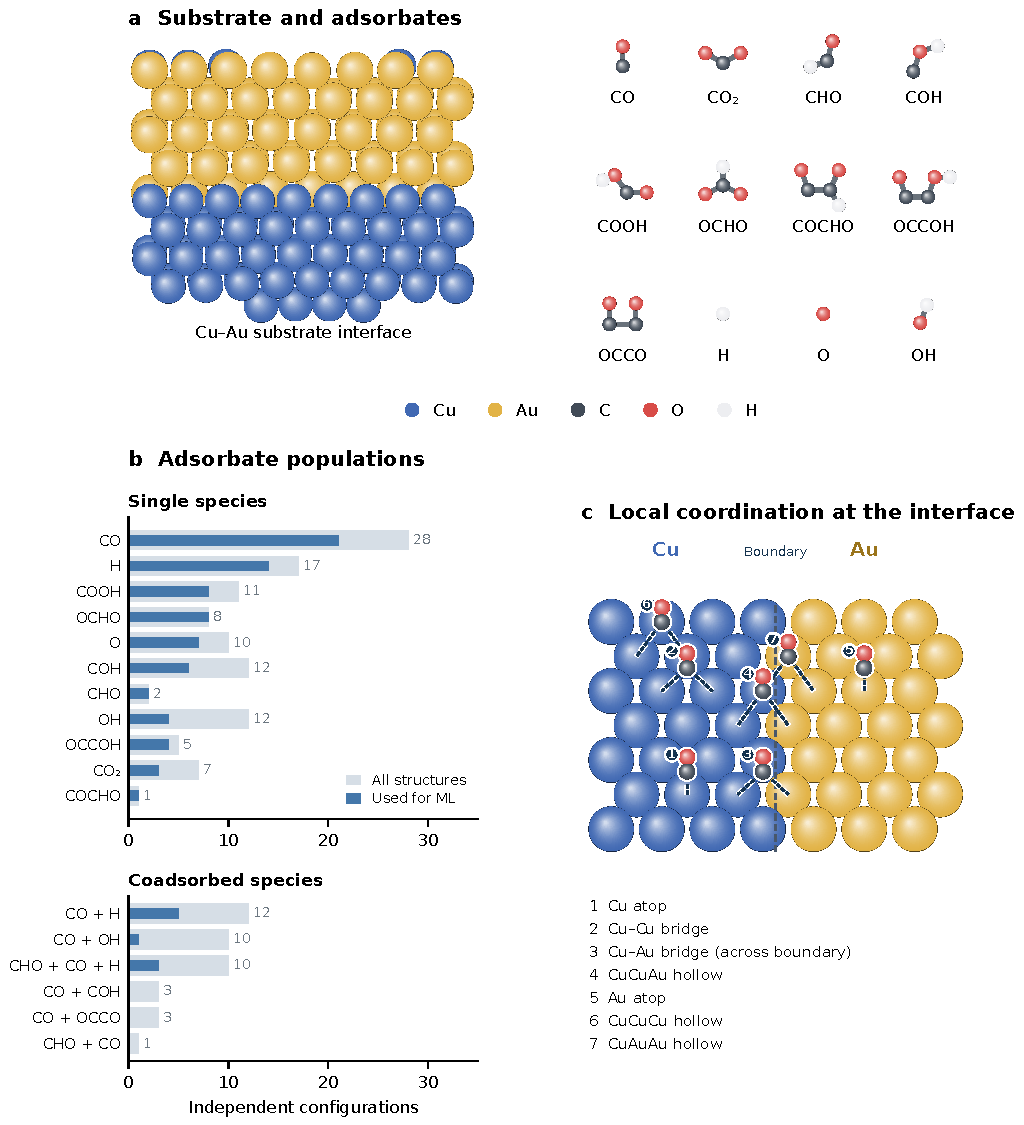
\includegraphics[width=\linewidth]{figures/Figure_2_dataset.pdf}
\caption{Chemical and structural variation at Cu--Au interfaces. (a) A shaded-atom rendering of a representative interfacial input and molecular templates covering the species in panel b. Cu, Au, C, O, and H are blue, gold, dark gray, red, and light gray. (b) Exclusive configuration counts, separated into single-species and coadsorbed states, for the full inventory and completed ML dataset. A single-species state can contain several molecules of that species. Two clean surfaces and one CuO reference are omitted from these adsorbate counts. (c) Seven CO adsorption motifs on one extended, schematic Cu--Au surface, with the adsorbates and metal lattice shown in the same oblique projection. The boundary-spanning bridge and three hollow compositions distinguish local metal coordination from interface proximity. Numbered sites and dashed metal-contact lines define the construction; the diagram does not represent relaxed geometries.}
\label{fig:dataset}
\end{figure}

The Cu--Au construction space includes pure Cu(111) and Au(111) surfaces and lateral stripe ratios of 1:1, 2:1, 1:2, 3:1, and 1:3. Explicit row counts define the parent model, while adsorption positions distinguish boundary, neighboring-row, and terrace environments. These are the available structural controls; the completed cohort samples a subset of their combinations. At each location, coverage and spatial distribution determine how many metal environments are perturbed and whether adsorbates have nearby reaction partners. Molecular coverage is therefore retained together with its reference surface population. Carbon-equivalent coverage provides an additional comparison for OCCO and spectator CO, permitting equal carbon loading to be maintained when two CO molecules form one coupled intermediate.

Equal loading does not, however, imply equal chemical identity. Neighboring CO molecules remain an uncoupled state unless a C--C bond forms; separate CO and H likewise differ from bonded CHO. Molecular connectivity and metal contacts are checked after relaxation so that the spectral label describes the state actually calculated. Single-species and coadsorbed configurations are distinguished in Fig.~\ref{fig:dataset}b. Together, these controls make the dataset suitable for asking which spectral differences arise from chemistry and which arise from changes in the surrounding interface.

\subsection{Preserving the information needed for a hypothesis test}
The records carry the information needed to decide whether two spectra constitute a controlled comparison. Adsorbate identity and molecular count specify the chemical alternatives; local coordination, interface distance, and coverage identify possible confounding changes. Absorber populations and calculation settings define how those structures contribute to the computed signal. Retaining these quantities together allows spectra to be regrouped for a new question without reconstructing their meaning from filenames. Coadsorption is treated as simultaneous species presence: CO+H contains two labels, while bonded CHO is a distinct molecular label. Structural descriptors define targets and support quality control; the classifiers reported here receive spectral features only.

A second hypothesis concerns observability: a real intermediate can be spectroscopically difficult to detect if most absorbers are far from it. Layer-resolved spectra separate this dilution question from changes in adsorbate identity. They permit surface and subsurface contributions to be examined for the same configuration. For layer means $\mu_l(E)$ representing $n_l$ Cu sites, a combined representation is formed as
\begin{equation}
\mu_D(E)=\frac{\sum_{l\in D}n_l\mu_l(E)}{\sum_{l\in D}n_l}.
\label{eq:average}
\end{equation}
Population weighting precedes spectral normalization. This preserves the physical meaning of a layer average and avoids assigning equal contributions to ensembles containing different numbers of absorbers. The same configuration is then evaluated through individual-layer and combined-layer representations, allowing depth sensitivity to be compared without changing the underlying sample population.

\section{Results and discussion}
\subsection{Simulation and evaluation design}
The \ca{} structures were relaxed using VASP, and the completed identity benchmark uses convolved Cu K-edge spectra calculated with the Green-function multiple-scattering mode of FDMNES.\cite{vasp1996,joly2001} The Green-function treatment provides a practical route to sampling many absorber environments; its muffin-tin approximation reduces computational cost relative to the finite-difference treatment.\cite{fdmnesmanual} The new numeric reference comparison supports this practical choice for metallic Cu and Cu\textsubscript{2}O under the disclosed short-window processing: common-offset normalized RMSE is 0.054/0.103 for Green and 0.090/0.107 for finite differences, respectively (Section~3.3 and SI). This is a conditional accuracy--cost tradeoff, not a universal ranking. For Cu\textsubscript{2}O, finite differences slightly outperform Green after separate shape alignment (0.1019 versus 0.1023) and under the extra-Gaussian sensitivity (0.100 versus 0.102). The CuO finite-difference run lacks a completed native convolution, so its larger residual cannot establish a fair solver ranking. Timing logs have different or incompletely specified resources; the cost argument remains the documented qualitative one rather than a measured speedup. The available interface spectra sample four Cu layers, numbered 2--5, with layer 5 at the physical surface. We compare those individual layers and population-weighted averages of the top two, top three, and all four available layers. The four-layer average describes the sampled slab region rather than a macroscopic experimental ensemble.

The feature labels in Fig.~\ref{fig:ml}d denote five representations of the same spectrum. \textit{Normalized energy spectrum} is the minimum-subtracted, unit-area-normalized intensity sampled on the recorded energy grid; the photon-energy axis is not rescaled. \textit{CDF} is its cumulative integral, describing how spectral weight accumulates across the edge. \textit{d1} is the first energy derivative, emphasizing slopes and local changes. \textit{Combined} concatenates the smoothed normalized spectrum, CDF, and first and second derivatives. \textit{DCT24} retains the first 24 orthonormal type-II discrete-cosine-transform coefficients. The DCT expresses a sampled signal in cosine basis functions,\cite{ahmed1974} providing a compact alternative to the full energy-grid representation. The number 24 is the fixed feature dimension used in this study, not a physically defined cutoff or a value prescribed by the cited transform paper. Numerical definitions and smoothing parameters are given in the Supporting Information. Additional tree-based candidates retain separate surface and depth-contrast information. Candidate models include logistic regression, a radial-basis-function support-vector machine, random forests, joint extremely randomized trees, and independent binary tree ensembles for each adsorbate.\cite{geurts2006} Adsorbate identity is a multilabel task; neither coverage nor geometry is predicted in this benchmark.

Five outer folds hold out entire configurations, and three inner folds select features and decision thresholds from each outer-training partition. All layer spectra from a configuration remain together. Learned preprocessing is fitted using training data only. The primary automated procedure selects independent-species tree representations within the training folds. Performance is summarized by pooled held-out micro F1, macro F1 across the 11 species, and exact identity-set accuracy. A separate comparison of fixed feature/model combinations is exploratory. Conditional confidence intervals are obtained by resampling the held-out configurations. Computational parameters, label checks, model settings, fold assignments, and the interval calculation are detailed in the Supporting Information.

For species $s$, precision and recall are $P_s=TP_s/(TP_s+FP_s)$ and $R_s=TP_s/(TP_s+FN_s)$, where $TP$, $FP$, and $FN$ count true-positive, false-positive, and false-negative configuration--species assignments. The reported scores are
\begin{align}
F_{1,\mathrm{micro}}&=\frac{2\sum_s TP_s}{2\sum_s TP_s+\sum_s FP_s+\sum_s FN_s},\\
F_{1,\mathrm{macro}}&=\frac{1}{S}\sum_{s=1}^{S}\frac{2TP_s}{2TP_s+FP_s+FN_s},\\
A_{\mathrm{set}}&=\frac{1}{N}\sum_{i=1}^{N}\mathbf{1}\!\left[\widehat{\boldsymbol y}_i=\boldsymbol y_i\right].
\end{align}
Here $S=11$ species and $N=87$ configurations; undefined species-level scores are assigned zero. Micro F1 emphasizes the recovered assignments across the cohort, macro F1 weights species equally, and exact-set accuracy requires every species in a configuration to be correct. These measures distinguish detection of a dominant intermediate from complete recovery of a coadsorbed state.

\subsection{Chemical alternatives represented in the dataset}
The full inventory contains 155 distinct structures, including configurations whose calculations are still in progress. The completed benchmark contains 87 independent configurations with four compatible layer spectra each. Deduplication and chemical checks establish the statistical sample at the configuration level. The completed species span CO, \co{}, CHO, COH, COOH, OCHO, COCHO, OCCOH, H, O, and OH, including mixed adsorbate states (Fig.~\ref{fig:dataset}b).

CO and H are the most represented species, occurring in 30 and 22 configurations, respectively. Nine configurations contain multiple species: five CO+H, three CHO+CO+H, and one CO+OH. The other 78 configurations contain a single observed species. This diversity allows the inference problem to include coadsorption and relaxed chemical identity rather than only a set of isolated molecular templates. The species were chosen to represent chemically different branches of CO\textsubscript{2} reduction: COOH and OCHO distinguish hydrogenation/connectivity alternatives, CHO and COH distinguish where hydrogen binds, and COCHO and OCCOH extend the comparison to C\textsubscript{2} chemistry. H and OH describe coadsorbed environments that can alter the interpretation of a carbon-containing state. CO receives particular emphasis because it is a precursor to carbon coupling in Cu-based CO\textsubscript{2}RR.\cite{zhan2024,montoya2013} Two adjacent CO molecules and bonded OCCO contain the same C and O loading but represent different stages of a coupling hypothesis. Here 2CO denotes adjacent CO without a C--C bond, whereas OCCO denotes the bonded intermediate. Distinguishing these states tests sensitivity to carbon coupling rather than merely to carbon loading.

\subsection{Spectral response to chemical environment and depth}
Reference compounds connect the calculation-route choice to transfer beyond the interfacial training cohort. Figure~\ref{fig:spectroscopy}a compares numeric Cu, Cu\textsubscript{2}O, and CuO references; the complete three-compound, five-method grid is in the SI. The original oxide FDMNES directory names are reversed relative to their decks and logs, and are relabeled by the recorded solver. Three VASP slots lack numeric XAS output and remain blank. The retained ``GW'' labels denote directory aliases: the available inputs/output specify supercell core-hole calculations, without a verified GW or Bethe--Salpeter step.

A single shift fitted on metallic Cu is shared across compounds for each backend; both FDMNES solvers share the same offset. The experimental photon-energy column is retained as the anchor, although independent calibration metadata are absent. Native-axis and separately aligned comparisons are supplied in the SI; fitted alignment is not evidence of absolute energy agreement. With common offsets, Green gives local edge-jump normalized RMSE of 0.054, 0.103, and 0.138 for Cu, Cu\textsubscript{2}O, and CuO; FEFF gives 0.100, 0.249, and 0.212. These values are conditional on short pre-edge support and unequal native final-state broadening. They support Green as a practical sampling route while identifying oxide line-shape and processing limitations. They do not validate transfer to operating interfaces or catalytic pathways. The nominal metallic experimental column describes a 100~nm Cu electrode at $-0.4$~V in the supplied header; it is not documented as a certified bulk foil. Full settings, missing-series provenance, and all fitted degrees of freedom accompany the numeric results.

\begin{figure}[!htbp]
\centering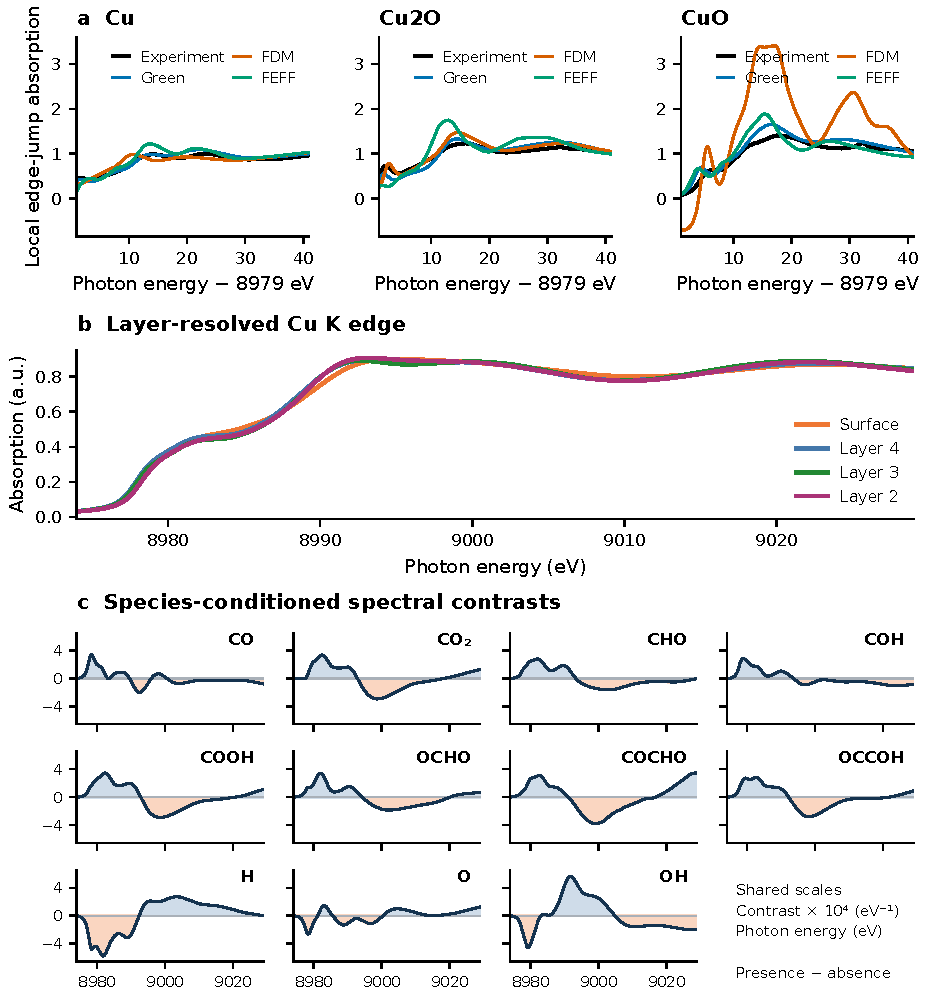
\includegraphics[width=\linewidth]{figures/Figure_3_spectroscopy.pdf}
\caption{Spectral sensitivity to reference chemistry, depth, and adsorbate identity. (a) Numeric Cu/Cu\textsubscript{2}O/CuO overlays for FDMNES and FEFF with common backend offsets fitted on Cu; VASP comparisons have dedicated space in the SI. Missing calculations are omitted from these compact overlays and left blank in the complete SI grid. The ``GW'' label is a folder alias, not a verified many-body treatment; the CuO FDM curve has only the added constant core lifetime, because its native convolution is absent. The reference normalization and alignment are separate from ML preprocessing. (b) Recorded layer-averaged Cu K-edge spectra for a CO-containing interfacial configuration. The outermost Cu layer is labeled surface. (c) Separate difference curves between mean normalized top-two-layer spectra for configurations containing each species and those without it, using common energy and amplitude scales. Blue and orange shading show positive and negative contrasts. These full-dataset contrasts include variation in coverage, geometry, and coadsorbates and are not unique molecular fingerprints.}
\label{fig:spectroscopy}
\end{figure}

The layer-resolved CO example retains a common broad metallic response while exhibiting smaller differences in the near-edge rise and higher-energy features (Fig.~\ref{fig:spectroscopy}b). These changes illustrate why a single averaged metal spectrum may conceal variation among physically distinct absorber environments. The local perturbation introduced by an adsorbate must be distinguished from the much larger spectral contribution shared across the slab.

Across the dataset, species-dependent mean contrasts are strongest in the early near-edge region, with additional differences at higher energies (Fig.~\ref{fig:spectroscopy}c). The separated maxima of the root-mean-square contrast occur at approximately 8978.8, 8981.8, 8991.2, and 8998.2~eV on the recorded simulation scale. H-containing configurations show a negative early-region contrast, whereas OH has a positive contrast near 8991~eV. Several carbon-containing species share similar broad patterns. Because coverage and geometry also vary across these groups, the separate curves identify regions of dataset-level contrast rather than assigning an isolated causal effect to each species.

\subsection{Automated adsorbate identification}
The primary independent-species tree selector achieves a pooled held-out micro F1 of 0.779 and macro F1 of 0.638, with exact identity-set accuracy of 0.690 (Fig.~\ref{fig:ml}a). The natural-language agent invoked the primary training procedure on the verified cohort, reproducing these held-out predictions in a fresh run. Models saved and reloaded for all five outer folds retained their held-out predictions. The inputs are simulated spectra alone, with model selection performed inside the training partitions. The higher micro than macro score indicates that common species are recovered more reliably than the dataset-wide average over species. A training-most-common-identity-set baseline, evaluated on the same outer folds, gives micro F1 0.323 and exact-set accuracy 0.241; the majority binary constant predicts no species and gives F1 zero. The improvement over these baselines shows that the spectra contain information beyond the most frequent labels. It does not by itself establish a unique mechanistic assignment.

\begin{figure}[!htbp]
\centering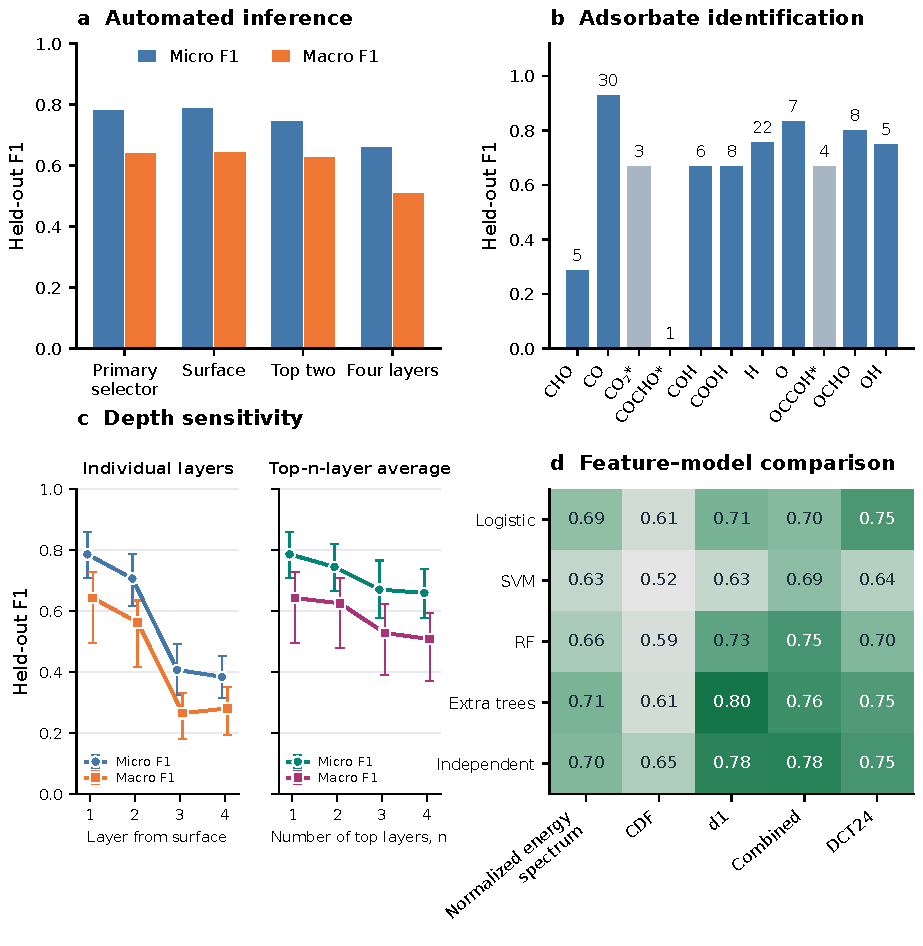
\includegraphics[width=\linewidth]{figures/Figure_4_ML.pdf}
\caption{Automated inference from simulated Cu K-edge spectra. (a) Pooled held-out micro and macro F1 for the primary and fixed-depth selectors. (b) Species-level F1; numbers give positive configuration counts, with asterisks for fewer than five positives. (c) Separate plots compare individual layers (left; layer 1 is the surface) and population-weighted means of the top $n$ layers (right). Thus $n=2$ combines the surface and its immediate subsurface layer. Error bars are conditional 95\% intervals from 1500 held-out bootstrap resamples. (d) Exploratory feature/model comparison for the surface layer. Normalized energy spectrum denotes normalized intensity on the energy grid; CDF, cumulative integral; d1, first derivative; Combined, concatenated spectrum/integral/derivative features; and DCT24, the first 24 cosine coefficients. Green indicates higher F1 and gray lower F1. Thresholds use training data; the highest observed fixed entry is exploratory.}
\label{fig:ml}
\end{figure}

CO reaches F1 0.929, with precision 1.000 and recall 0.867 over its 30 positive configurations. H reaches F1 0.757, while O and OCHO reach 0.833 and 0.800, respectively. CHO is more difficult, with F1 0.286 across five positives. The singleton COCHO case has no positive training counterpart when held out and receives F1 zero. Its result reflects a sampling constraint that cannot be resolved by increasing model complexity alone.

The fixed feature/model comparison identifies top-layer first derivatives with joint extra-trees as the strongest observed combination, with micro/macro F1 of 0.798/0.660 (Fig.~\ref{fig:ml}d). This result suggests that local shape variation is informative in the present dataset. Because the configuration was selected after comparing outer-fold scores, it provides a candidate recipe for subsequent validation. The primary nested selector remains the appropriate summary of the automated selection procedure.

Coadsorbate detection is a distinct challenge. For the exploratory fixed model, H is detected in all 14 single-species H configurations but in only one of eight H-containing mixtures. OH is detected in three of four single-species cases and zero of one mixture; CHO is detected in one of two single-species cases and zero of three mixtures. Thus successful recovery of the dominant adsorbate does not necessarily imply complete recovery of the surface identity set. Matched coadsorption calculations are especially valuable because they can separate the spectral response of a spectator species from changes in coverage and local binding.

\subsection{Surface sensitivity and signal dilution}
The same configuration folds distinguish two depth effects (Fig.~\ref{fig:ml}c): the information carried by each individual Cu layer, and its dilution when deeper layers are progressively included in an average. Individual-layer performance falls sharply away from the surface, whereas cumulative averages show a more gradual decrease. The micro F1 declines from 0.786 at the surface to 0.659 for the four-layer average (Table~\ref{tab:performance}). This difference is consistent with the strongest adsorbate-induced perturbations being localized near the exposed metal sites.

\begin{table}[!htbp]\centering\small
\caption{Depth-dependent inference with inner-selected features and thresholds. Scores are pooled over the same five outer configuration folds.}\label{tab:performance}
\begin{tabular}{@{}lccc@{}}\toprule
Spectral representation & Micro F1 & Macro F1 & Exact identity set\\\midrule
Surface layer &0.786&0.643&0.701\\
Top-two-layer average &0.744&0.625&0.621\\
Top-three-layer average &0.670&0.528&0.586\\
Four-layer average &0.659&0.508&0.529\\\bottomrule
\end{tabular}
\end{table}

The paired conditional 95\% interval for the surface-minus-four-layer micro F1 difference is 0.069--0.191. In contrast, the smaller surface-to-top-two difference has an interval crossing zero. Thus the data support loss of information on inclusion of deeper environments, without resolving a clear performance difference between the surface and the top-two-layer representation.

The result connects the statistical task to a physical measurement issue. Surface adsorbates perturb a subset of metal environments, whereas averaging adds contributions that contain less information about those adsorbates. The present slab averages isolate this effect within the simulated dataset. Experimental transfer additionally requires appropriate weighting for particle structure, orientation, attenuation, and detection mode; the four-layer slab representation alone does not determine an experimental probing depth.

\subsection{Formulating a carbon-coupling test at the interface}
The central catalytic hypothesis is that formation of a C--C-bonded intermediate produces a spectral change distinguishable from the presence of nearby CO, and that the Cu--Au boundary modifies that contrast. This hypothesis is motivated by the role of CO-derived dimers in proposed C\textsubscript{2} pathways.\cite{zhan2024,montoya2015} The structural controls permit a targeted comparison of two adjacent CO molecules with a bonded OCCO intermediate at equal C and O loading. The four starting models in Fig.~\ref{fig:coupling} combine coupled or uncoupled carbon with Cu-side interface or Cu-terrace placement. Their initial C--C separations are approximately 2.52 and 2.46~\AA{} for adjacent CO and 1.45~\AA{} for OCCO. Interface distance is varied while holding the parent cell and two-C/two-O loading fixed.

\begin{figure}[!htbp]
\centering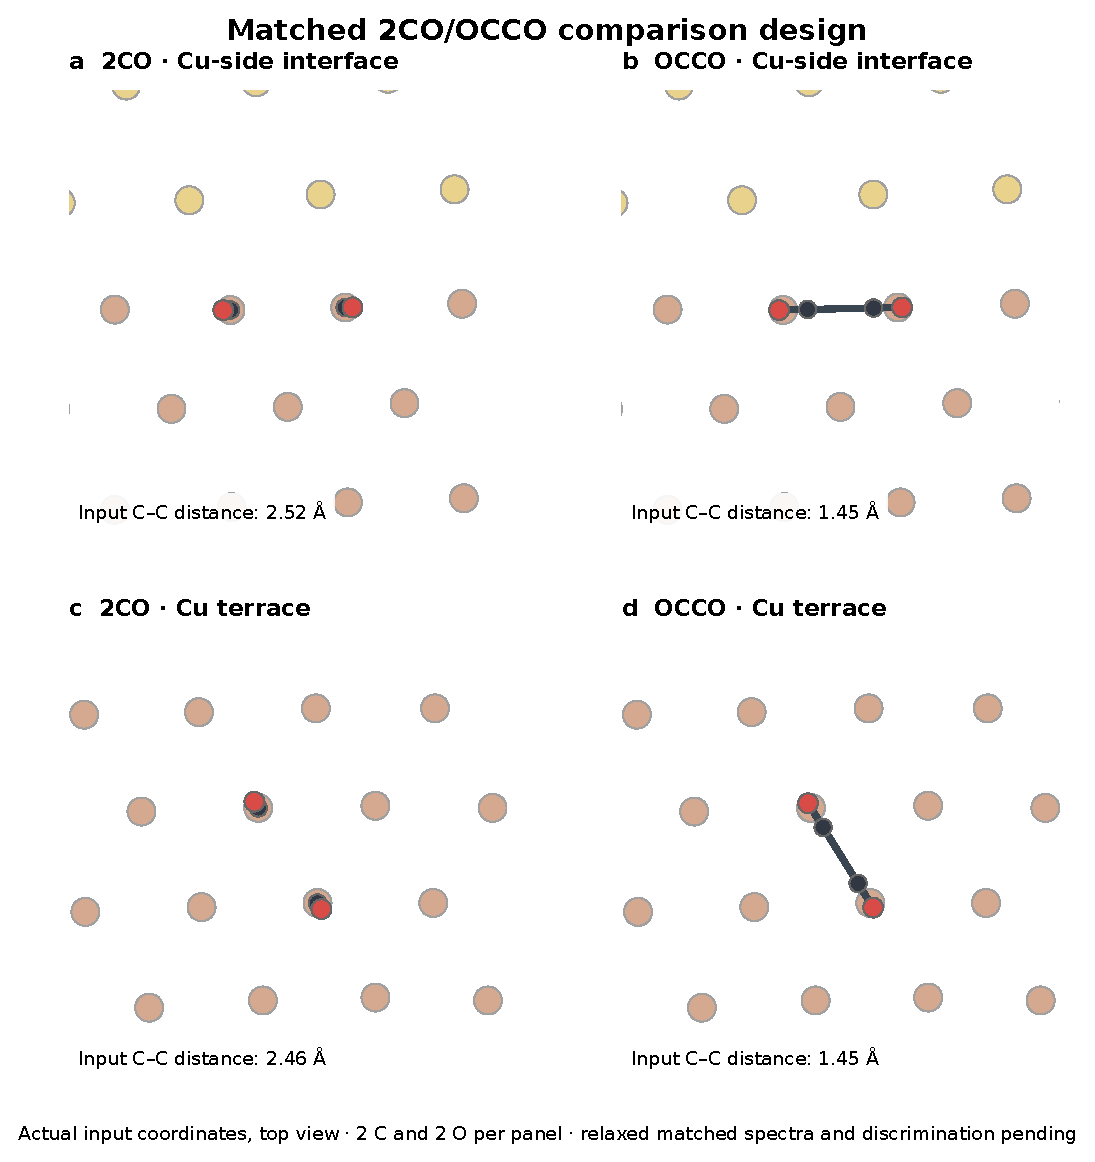
\includegraphics[width=.94\linewidth]{figures/Figure_5_CO_coupling.pdf}
\caption{Starting models for a matched carbon-coupling comparison. Adjacent CO and bonded OCCO are placed at a Cu-side interface or Cu terrace with identical elemental loading of two C and two O atoms. The structures use the actual input coordinates; reported C--C separations are initial values. Comparing their verified relaxed structures and spectra would separate changes associated with C--C bonding from those associated with interface location.}
\label{fig:coupling}
\end{figure}

This comparison addresses a specific spectroscopic question: does C--C bonding produce a resolvable response, and does that response depend on proximity to Au? Carbon coupling is sensitive to both surface structure and adsorbate state,\cite{montoya2013,montoya2015} making the matched design preferable to comparing unrelated examples at different loadings. The completed identity cohort does not contain intact-OCCO positives, so coupling-state discrimination is not inferred from its classification scores. Verified relaxed connectivity and matched Cu, C, and O spectra are needed to complete the test. For a fixed absorber definition, the interface-specific effect can be expressed as
\begin{equation}
\Delta\Delta\mu(E)=\left[\mu_{\rm OCCO}(E)-\mu_{\rm 2CO}(E)\right]_{\rm interface}
-\left[\mu_{\rm OCCO}(E)-\mu_{\rm 2CO}(E)\right]_{\rm terrace}.
\end{equation}
This difference of differences separates the coupling contrast from a response common to both chemical states at a given location. It is a defined analysis target, not a measured result in the present cohort. Spectral separation would establish sensitivity to the proposed structural states; a claim about reaction barriers or selectivity would require additional energetic or kinetic evidence.

\subsection{Implications for spectroscopy-guided catalyst analysis}
The workflow supports catalytic hypothesis testing at two levels. First, the completed identity and depth analyses establish whether a spectral channel can detect chemical alternatives and how ensemble averaging reduces that information. Second, matched calculations can test a proposed intermediate while controlling its elemental loading and local environment. A positive identity prediction narrows the structural alternatives; discrimination of a reaction step requires the second level of comparison. Adsorbate identity, local coordination, and absorber population determine the scientific meaning of the learning task. Preserving them throughout the workflow allows prediction errors to inform the next calculations: rare species require independent examples, coadsorbate omissions call for matched mixtures, and depth-dependent performance motivates more selective absorber representations.

The \ca{} demonstration establishes this approach within a simulated Cu K-edge dataset. Extension to other metal pairs requires new spectral validation even when the same structure builder can generate their interfaces. Likewise, configuration-level testing does not establish transfer to unseen parent structures, applied potentials, or experimental spectra. Energy alignment, broadening, noise, and the distributions sampled under reaction conditions remain central questions for transfer. Complementary edges and multimodal measurements offer a route to reduce ambiguities,\cite{jia2026} while robust featurization can help address differences between calculation and experiment.\cite{chen2024} The framework provides the structural controls and linked data needed to examine these questions systematically.

\section{Conclusions}
We have developed an end-to-end framework that connects catalytic hypotheses to interface construction, structural relaxation, NERSC-based XAS calculations, AI-ready records, and automated machine-learning analysis. The approach represents adsorbates through their local geometry and chemical identity and preserves the relation between each configuration and its derived spectra. In a simulation-only \ca{} demonstration, the automated selector reaches micro F1 0.779 for adsorbate identification. Performance decreases as deeper Cu layers enter the spectral average, linking inference directly to surface-signal dilution. These results establish the feasibility of recovering adsorbate information and define the absorber populations most informative for testing a surface-chemistry hypothesis. The matched 2CO/OCCO design makes the next mechanistic question explicit: whether bonding and interface location produce separable spectral contrasts at fixed loading. Matched coadsorption states, complementary edges, and verified coupled/uncoupled configurations provide natural extensions toward spectroscopy-based tests of catalytic mechanisms.

\section*{Data availability}
The agent implementation and analysis outputs are available at \url{https://github.com/HailiJia/CO2RR_XAS_agent}. Figure-generation scripts and the plotted data accompany this manuscript.

\begin{thebibliography}{99}
\bibitem{ni2024} W. Ni, H. Chen, N. Tang \textit{et al.}, High-purity ethylene production via indirect carbon dioxide electrochemical reduction, \textit{Nat. Commun.}, 2024, \textbf{15}, 6078, DOI: \href{https://doi.org/10.1038/s41467-024-50522-7}{10.1038/s41467-024-50522-7}.
\bibitem{francis2018} S. A. Francis, J. M. Velazquez, I. M. Ferrer, D. A. Torelli, D. Guevarra, M. T. McDowell, K. Sun, X. Zhou, F. H. Saadi, J. John, M. H. Richter, F. P. Hyler, K. M. Papadantonakis, B. S. Brunschwig and N. S. Lewis, Reduction of aqueous CO\textsubscript{2} to 1-propanol at MoS\textsubscript{2} electrodes, \textit{Chem. Mater.}, 2018, \textbf{30}, 4902--4908, DOI: \href{https://doi.org/10.1021/acs.chemmater.7b04428}{10.1021/acs.chemmater.7b04428}.
\bibitem{zhan2024} C. Zhan, F. Dattila, C. Rettenmaier, A. Herzog, M. Herran, T. Wagner, F. Scholten, A. Bergmann, N. L\'opez and B. Roldan Cuenya, Key intermediates and Cu active sites for CO\textsubscript{2} electroreduction to ethylene and ethanol, \textit{Nat. Energy}, 2024, \textbf{9}, 1485--1496, DOI: \href{https://doi.org/10.1038/s41560-024-01633-4}{10.1038/s41560-024-01633-4}.
\bibitem{montoya2015} J. H. Montoya, C. Shi, K. Chan and J. K. N\o rskov, Theoretical insights into a CO dimerization mechanism in CO\textsubscript{2} electroreduction, \textit{J. Phys. Chem. Lett.}, 2015, \textbf{6}, 2032--2037, DOI: \href{https://doi.org/10.1021/acs.jpclett.5b00722}{10.1021/acs.jpclett.5b00722}.
\bibitem{operando2021} J. Timoshenko and B. Roldan Cuenya, In situ/operando electrocatalyst characterization by X-ray absorption spectroscopy, \textit{Chem. Rev.}, 2021, \textbf{121}, 882--961, DOI: \href{https://doi.org/10.1021/acs.chemrev.0c00396}{10.1021/acs.chemrev.0c00396}.
\bibitem{lin2020} S.-C. Lin, C.-C. Chang, S.-Y. Chiu, H.-T. Pai, T.-Y. Liao, C.-S. Hsu, W.-H. Chiang, M.-K. Tsai and H. M. Chen, Operando time-resolved X-ray absorption spectroscopy reveals the chemical nature enabling highly selective CO\textsubscript{2} reduction, \textit{Nat. Commun.}, 2020, \textbf{11}, 3525, DOI: \href{https://doi.org/10.1038/s41467-020-17231-3}{10.1038/s41467-020-17231-3}.
\bibitem{morales2018} C. G. Morales-Guio, E. R. Cave, S. A. Nitopi, J. T. Feaster, L. Wang, K. P. Kuhl, A. Jackson, N. C. Johnson, D. N. Abram, T. Hatsukade, C. Hahn and T. F. Jaramillo, Improved CO\textsubscript{2} reduction activity towards C\textsubscript{2+} alcohols on a tandem gold on copper electrocatalyst, \textit{Nat. Catal.}, 2018, \textbf{1}, 764--771, DOI: \href{https://doi.org/10.1038/s41929-018-0139-9}{10.1038/s41929-018-0139-9}.
\bibitem{rehr2010} J. J. Rehr, J. J. Kas, F. D. Vila, M. P. Prange and K. Jorissen, Parameter-free calculations of X-ray spectra with FEFF9, \textit{Phys. Chem. Chem. Phys.}, 2010, \textbf{12}, 5503--5513, DOI: \href{https://doi.org/10.1039/B926434E}{10.1039/B926434E}.
\bibitem{joly2001} Y. Joly, X-ray absorption near-edge structure calculations beyond the muffin-tin approximation, \textit{Phys. Rev. B}, 2001, \textbf{63}, 125120, DOI: \href{https://doi.org/10.1103/PhysRevB.63.125120}{10.1103/PhysRevB.63.125120}.
\bibitem{vasp1996} G. Kresse and J. Furthm\"uller, Efficient iterative schemes for ab initio total-energy calculations using a plane-wave basis set, \textit{Phys. Rev. B}, 1996, \textbf{54}, 11169--11186, DOI: \href{https://doi.org/10.1103/PhysRevB.54.11169}{10.1103/PhysRevB.54.11169}.
\bibitem{vaspxas} VASP Wiki, Supercell core-hole calculations, \url{https://vasp.at/wiki/index.php/SCH_calculations}, accessed 21 October 2026.
\bibitem{ocean2011} J. Vinson, J. J. Rehr, J. J. Kas and E. L. Shirley, Bethe--Salpeter equation calculations of core excitation spectra, \textit{Phys. Rev. B}, 2011, \textbf{83}, 115106, DOI: \href{https://doi.org/10.1103/PhysRevB.83.115106}{10.1103/PhysRevB.83.115106}.
\bibitem{timoshenko2018} J. Timoshenko, A. Anspoks, A. Cintins, A. Kuzmin, J. Purans and A. I. Frenkel, Neural network approach for characterizing structural transformations by X-ray absorption fine structure spectroscopy, \textit{Phys. Rev. Lett.}, 2018, \textbf{120}, 225502, DOI: \href{https://doi.org/10.1103/PhysRevLett.120.225502}{10.1103/PhysRevLett.120.225502}.
\bibitem{marcella2020} N. Marcella, Y. Liu, J. Timoshenko, E. Guan, M. Luneau, T. Shirman, A. M. Plonka, J. E. S. van der Hoeven, J. Aizenberg, C. M. Friend and A. I. Frenkel, Neural network assisted analysis of bimetallic nanocatalysts using X-ray absorption near edge structure spectroscopy, \textit{Phys. Chem. Chem. Phys.}, 2020, \textbf{22}, 18902--18910, DOI: \href{https://doi.org/10.1039/D0CP02098B}{10.1039/D0CP02098B}.
\bibitem{torrisi2020} S. B. Torrisi, M. R. Carbone, B. A. Rohr, J. H. Montoya, Y. Ha, J. Yano, S. K. Suram and L. Hung, Random forest machine learning models for interpretable X-ray absorption near-edge structure spectrum-property relationships, \textit{npj Comput. Mater.}, 2020, \textbf{6}, 109, DOI: \href{https://doi.org/10.1038/s41524-020-00376-6}{10.1038/s41524-020-00376-6}.
\bibitem{david2023} T. David, N. K. Nik Aznan, K. Garside and T. J. Penfold, Towards the automated extraction of structural information from X-ray absorption spectra, \textit{Digital Discovery}, 2023, \textbf{2}, 1461--1470, DOI: \href{https://doi.org/10.1039/D3DD00101F}{10.1039/D3DD00101F}.
\bibitem{chen2024} Y. Chen, C. Chen, I. Hwang, M. J. Davis, W. Yang, C. Sun, G.-H. Lee, D. McReynolds, D. Allan, J. Marulanda Arias, S. P. Ong and M. K. Y. Chan, Robust machine learning inference from X-ray absorption near edge spectra through featurization, \textit{Chem. Mater.}, 2024, \textbf{36}, 2304--2313, DOI: \href{https://doi.org/10.1021/acs.chemmater.3c02584}{10.1021/acs.chemmater.3c02584}.
\bibitem{jia2026} H. Jia, Y. Chen, G.-H. Lee, J. Smith, M. Chi, W. Yang and M. K. Y. Chan, Revealing local structures through machine-learning-fused multimodal spectroscopy, \textit{ACS Nano}, 2026, \textbf{20}, 4228--4240, DOI: \href{https://doi.org/10.1021/acsnano.5c16942}{10.1021/acsnano.5c16942}.
\bibitem{bran2024} A. M. Bran, S. Cox, O. Schilter, C. Baldassari, A. D. White and P. Schwaller, Augmenting large language models with chemistry tools, \textit{Nat. Mach. Intell.}, 2024, \textbf{6}, 525--535, DOI: \href{https://doi.org/10.1038/s42256-024-00832-8}{10.1038/s42256-024-00832-8}.
\bibitem{canty2023} R. B. Canty, B. A. Koscher, M. A. McDonald and K. F. Jensen, Integrating autonomy into automated research platforms, \textit{Digital Discovery}, 2023, \textbf{2}, 1259--1268, DOI: \href{https://doi.org/10.1039/D3DD00135K}{10.1039/D3DD00135K}.
\bibitem{vriza2026} A. Vriza \textit{et al.}, Multi-agentic AI framework for end-to-end atomistic simulations, \textit{Digital Discovery}, 2026, \textbf{5}, 440--452, DOI: \href{https://doi.org/10.1039/D5DD00435G}{10.1039/D5DD00435G}.
\bibitem{nersc} NERSC, The Superfacility API, \url{https://docs.nersc.gov/services/sfapi/}, accessed 21 October 2026.
\bibitem{fdmnesmanual} Y. Joly, \textit{FDMNES User's Guide}, November 2022, \url{https://data-analysis.synchrotron-soleil.fr/tmp/software/fdmnes/fdmnes_Linux/Doc/Manual_Eng.pdf}, accessed 21 October 2026.
\bibitem{ahmed1974} N. Ahmed, T. Natarajan and K. R. Rao, Discrete cosine transform, \textit{IEEE Trans. Comput.}, 1974, \textbf{C-23}, 90--93, DOI: \href{https://doi.org/10.1109/T-C.1974.223784}{10.1109/T-C.1974.223784}.
\bibitem{geurts2006} P. Geurts, D. Ernst and L. Wehenkel, Extremely randomized trees, \textit{Mach. Learn.}, 2006, \textbf{63}, 3--42, DOI: \href{https://doi.org/10.1007/s10994-006-6226-1}{10.1007/s10994-006-6226-1}.
\bibitem{montoya2013} J. H. Montoya, A. A. Peterson and J. K. N\o rskov, Insights into C--C coupling in CO\textsubscript{2} electroreduction on copper electrodes, \textit{ChemCatChem}, 2013, \textbf{5}, 737--742, DOI: \href{https://doi.org/10.1002/cctc.201200564}{10.1002/cctc.201200564}.
\end{thebibliography}

\end{document}
